\documentclass{beamer}

\usepackage[T1]{fontenc}
\usepackage{lmodern}
\usepackage{microtype}
\usepackage[size=custom,width=120,height=72,scale=1.0]{beamerposter}
\usepackage{graphicx}
\usepackage{booktabs}
\usepackage[numbers]{natbib}
\usepackage{tikz}
\usepackage{pgfplots}
\usepackage{calc}
% \usepackage{anyfontsize}

\usetheme{gemini}
\usecolortheme{cam}

\pgfplotsset{compat=1.14}
\usetikzlibrary{arrows.meta,positioning,fit,backgrounds}

\newlength{\sepwidth}
\setlength{\sepwidth}{0.025\paperwidth}

% \newlength{\colwidth}
% \setlength{\colwidth}{0.3\paperwidth}

\newlength{\centerwidth}
\setlength{\centerwidth}{0.5\paperwidth}

\newlength{\edgewidth}
\setlength{\edgewidth}{(\paperwidth - \centerwidth - 4\sepwidth) / 2}

\newcommand{\separatorcolumn}{\begin{column}{\sepwidth}\end{column}}

\tikzset{
	clause/.style={draw,thick,rounded corners=2pt,fill=white,inner xsep=8pt,inner ysep=6pt},
	core/.style={fill=camblue!20},
	panel/.style={draw,thick,rounded corners=4pt,fill=black!4},
	heading/.style={font=\Large\bfseries},
	flow/.style={-{Latex[length=24pt,width=36pt]},line width=8pt,camblue}
}

\newcommand{\flowarrow}{{\centering\tikz\draw[flow] (0pt,0pt) -- (0pt,-40pt);\par}}

\newcommand{\sidearrow}{\tikz\draw[flow] (0pt,0pt) -- (40pt,0pt);}

\newcommand{\diagram}[2]{\centering\vspace{16pt}\resizebox{#1\textwidth}{!}{\input{tikz/#2.tikz}}}

\newcommand{\cop}[1]{\textsf{\textbf{#1}}}

\title{All Axioms are Equal, but Some are More Equal than Others: \\ \huge Predicting relevance of first-order axioms }

\author{Martin S.\ Fixman\inst{1} \and Fredrik Rømming \inst{2} \and Sean Holden \inst{3}}

\newcommand{\crest}[1]{\raisebox{-0.5em}{\includegraphics[height=1.8em]{logos/#1-shield.pdf}}}

\institute[shortinst]{\inst{1} Hughes Hall \crest{hughes-hall} \hspace{1em} \inst{2} Emmanuel College \crest{emmanuel} \hspace{1em} \inst{3} Trinity College \crest{trinity} }

\footercontent{
	% \href{https://www.example.com}{https://www.example.com} \hfill
	\hfill
	\href{mailto:msf43@cl.cam.ac.uk}{msf43@cl.cam.ac.uk}
}

\begin{document}

\addtobeamertemplate{headline}{}
{
\begin{tikzpicture}[remember picture,overlay]
	\node [anchor=north west, inner sep=3cm] at ([xshift=0.0cm,yshift=1.0cm]current page.north west)
	{
\includegraphics[height=4.5cm]{logos/cambridge-reversed-color-logo.eps}};
	\node [anchor=north east, inner sep=0pt, opacity=0.5] at ([xshift=-350pt,yshift=-16pt]current page.north east)
	{
\includegraphics[height=280pt]{pictures/Napoleon.png}};
\end{tikzpicture}
}

\begin{frame}[t]
\begin{columns}[t]
	\separatorcolumn

	\begin{column}{\edgewidth}
		\begin{minipage}[t][1266pt][t]{\textwidth}
	\begin{block}{Every Axiom Makes the Search Harder}
		\Large
		TPTP problems have up to 3 million axioms~\cite{sutcliffe2017tptp}: many candidate solutions to a problem.
	\end{block}

	\vfill

	\begin{block}{Only a Few Axioms Matter}
		\Large
		{\diagram{1}{facts}\par}

		\vspace{16pt}

		{\centering A prover only learns which axioms \\ matter after finding the proof.\par}
	\end{block}

	\vfill

	\begin{exampleblock}{Our Goal}
		\Large
		\vspace{14pt}

		{\centering Predict which axioms matter \\ before the search begins.\par}
	\end{exampleblock}
\end{minipage}

	\end{column}

	\separatorcolumn

	\begin{column}{\centerwidth}

		\begin{block}{First-Order TPTP Problem \cop{SYN054+1}: Do the Axioms Prove the Conjecture?}
			\diagram{0.95}{problem}
		\end{block}

		\flowarrow

		\begin{block}{SAT Cores Label Relevant Axioms}
			\diagram{0.95}{tree}
		\end{block}

		\flowarrow

		\begin{columns}[T,totalwidth=\textwidth]
			\begin{column}{0.5\textwidth}
				\begin{block}{Train a Neural Network on Which \\ Axioms Contribute to the SAT Core}
					{\diagram{0.95}{network}\par}

					{\footnotesize\textsuperscript{*} The GNN comes from Rømming et al., \emph{Imitation Learning for Connection-Tableau Construction} \cite{romming2026imitation}.\par}
				\end{block}
			\end{column}

			\begin{column}{0.04\textwidth}
				\vspace{226pt}
				\sidearrow
			\end{column}

			\begin{column}{0.46\textwidth}
				\begin{block}{Relevance $p_x$ of \\ Each Axiom Clause}
					\centering
					\vspace{16pt}
					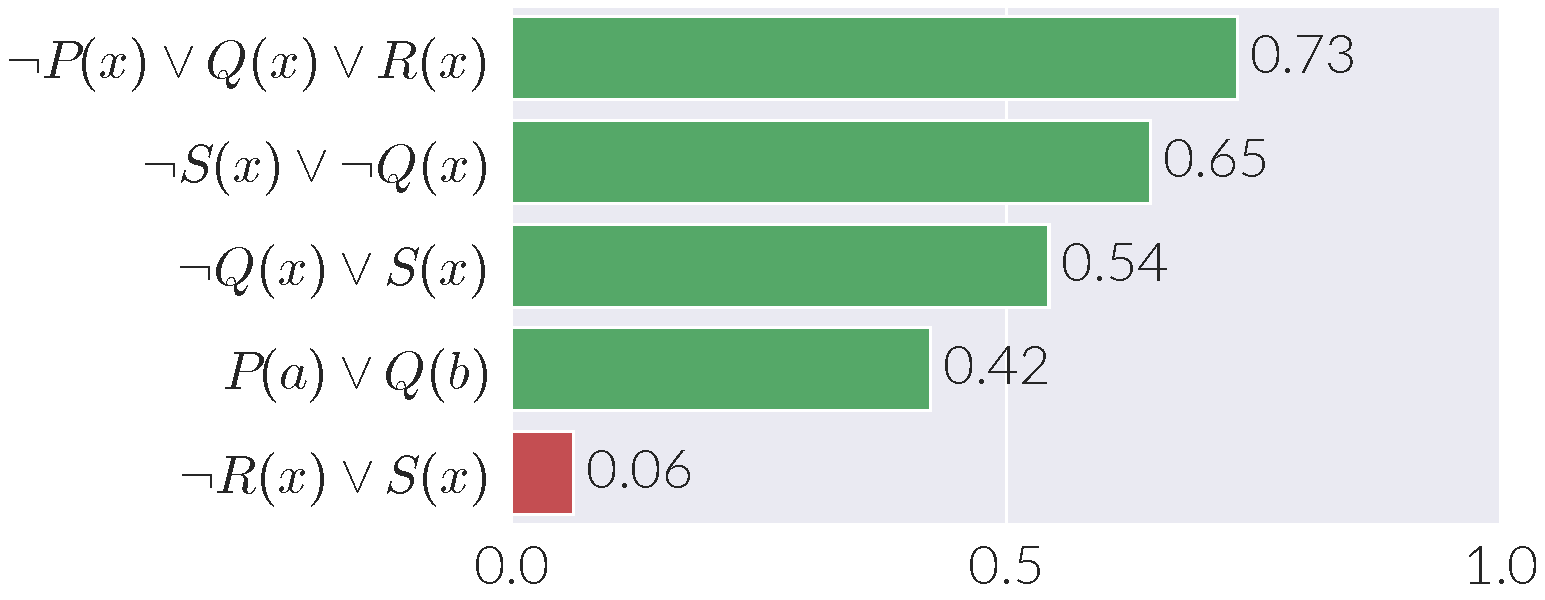
\includegraphics[width=0.95\textwidth]{figures/relevance.pdf}
				\end{block}
			\end{column}
		\end{columns}

		\flowarrow

	\end{column}

	\separatorcolumn

	\begin{column}{\edgewidth}
		\begin{minipage}[t][1270pt][t]{\textwidth}
	\begin{exampleblock}{Core Good, Non-Core Bad?}
		\large
		\vspace{14pt}

		Premise selection usually relies on symbol heuristics like SInE \cite{hoder2011sine}, or learns from formal libraries \cite{wang2017premise}.
		We learn from the prover's own refutations, like NeuroCore \cite{selsam2019neurocore} for SAT.
		Unlike neural clause selection \cite{chvalovsky2026teaching}, we only score the input axioms.

		An axiom outside the core was only unused in this proof, so we run the search on multiple seeds to find the widest variety of unsatisfiable subsets of axioms.

		{\diagram{0.9}{cores}\par}
	\end{exampleblock}

	\vfill

	\begin{block}{References}
		\renewcommand{\bibsection}{}
		\vspace{-8pt}
		\small{\bibliographystyle{abbrvnat}\bibliography{poster}}
	\end{block}
\end{minipage}

	\end{column}

	\separatorcolumn
\end{columns}

\begin{block}{Results: Guiding First-Order Provers (Higher is Better)}
	\centering
	\vspace{-52pt}
\makebox[\textwidth]{\parbox{\dimexpr\paperwidth-2\sepwidth\relax}{\raggedleft\footnotesize SATResetCoP: 120 seconds, 1 million steps. Prover9 and Vampire: 30 seconds. Models were trained, validated, and tested on separate sets of problems.}}
\vspace{-12pt}

\makebox[\textwidth]{\parbox{\dimexpr\paperwidth-2\sepwidth\relax}{
	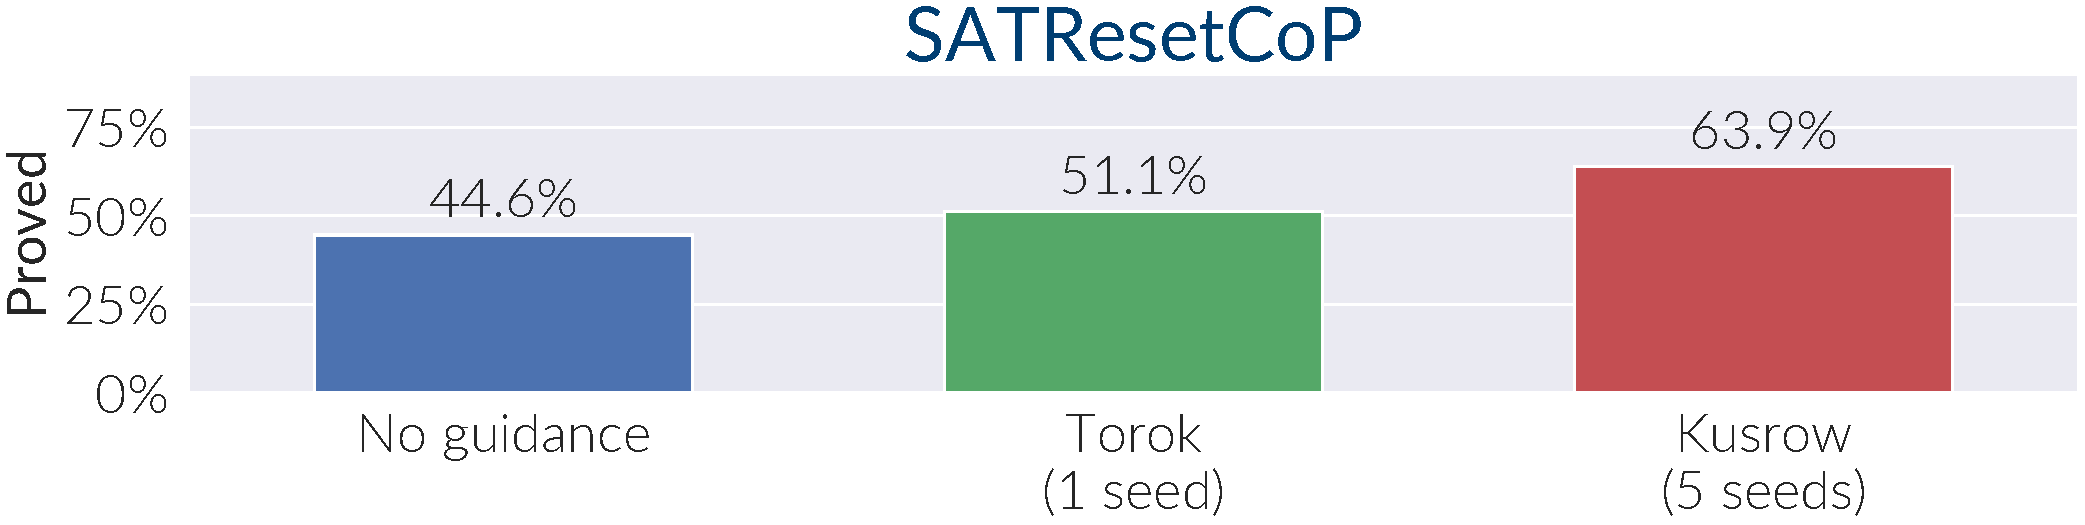
\includegraphics[width=0.31\linewidth]{figures/results-satresetcop.pdf}
	\hfill
	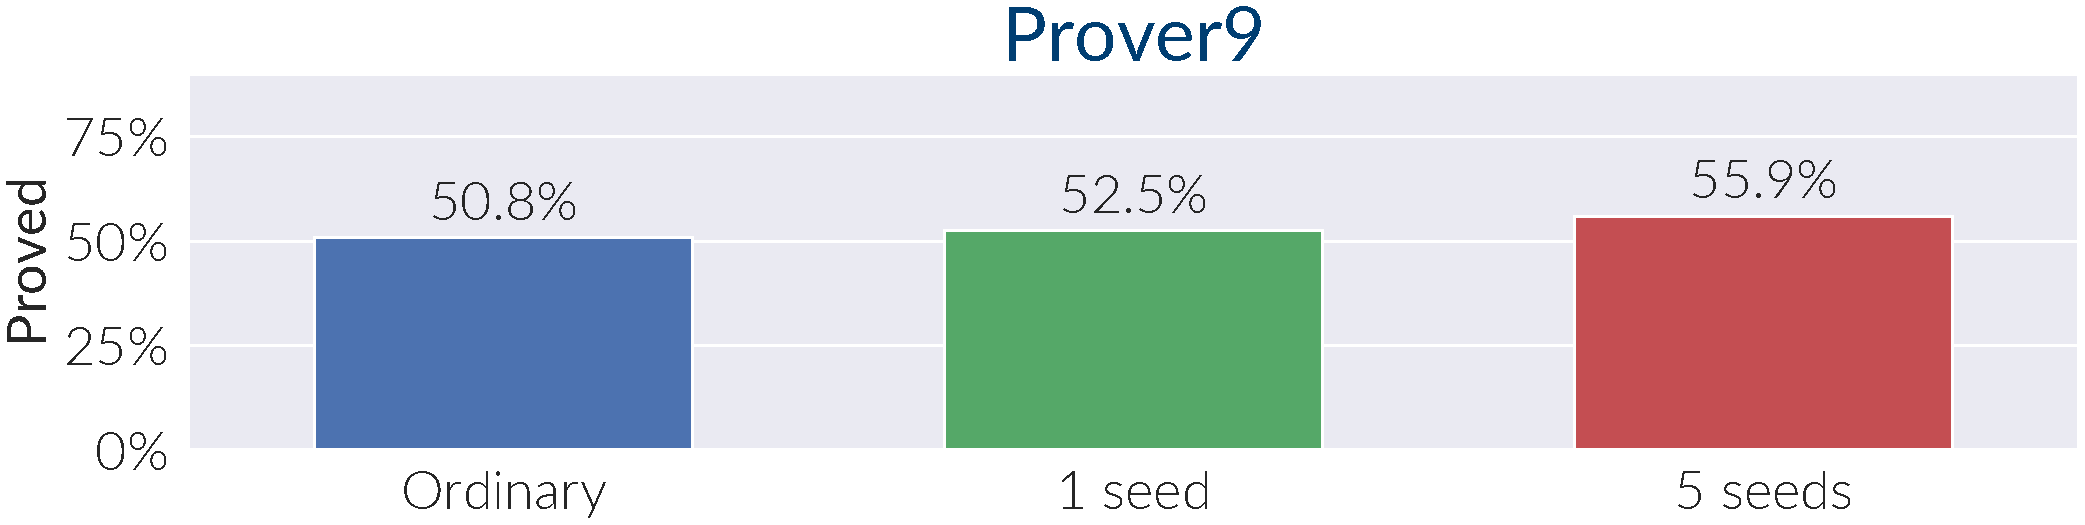
\includegraphics[width=0.31\linewidth]{figures/results-prover9.pdf}
	\hfill
	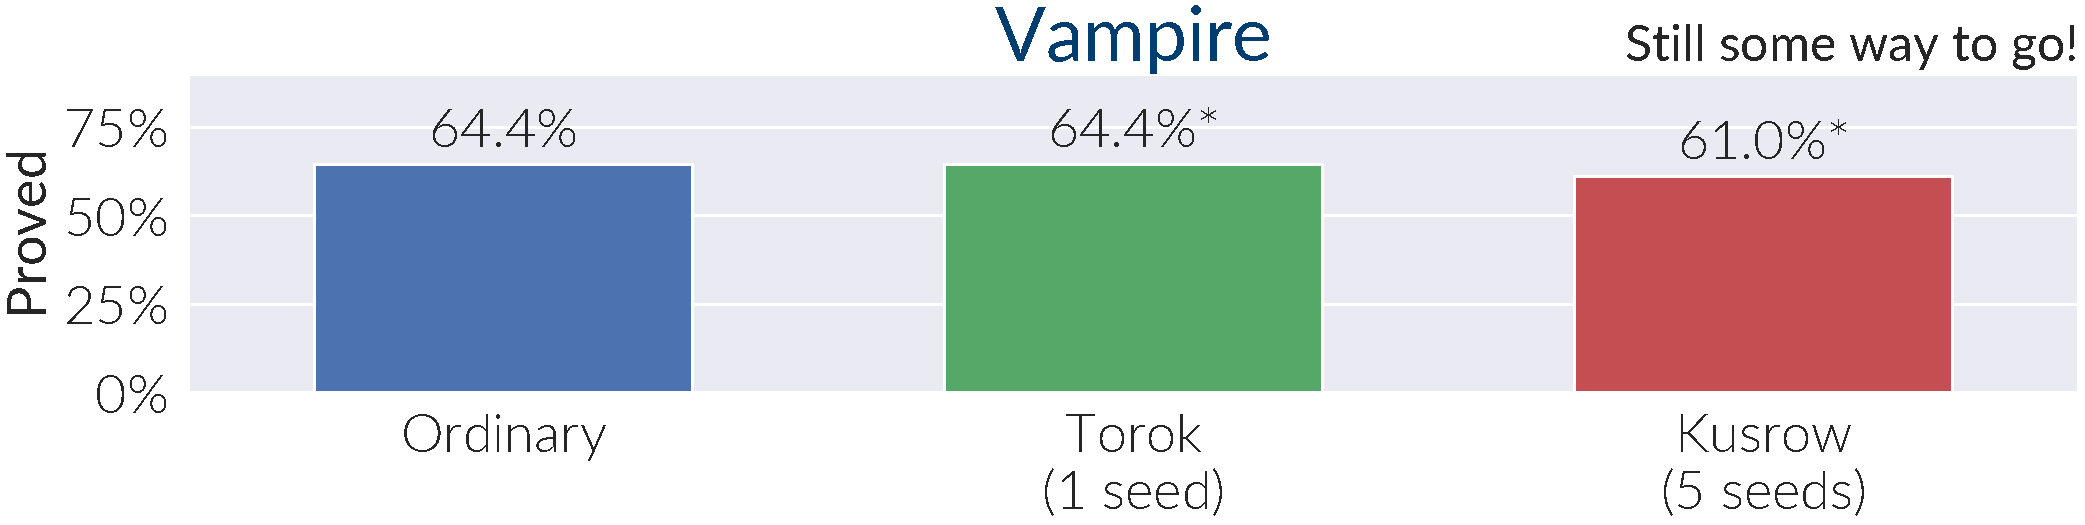
\includegraphics[width=0.31\linewidth]{figures/results-vampire.pdf}
}}

\end{block}

\end{frame}

\end{document}
